\chapter{Results}

Chapter \ref{chap:methods} builds three solvers. This chapter evaluates each of the three solvers and compares them against one another. 

\section{Experimental Setup:}
All models are evaluated on the same held out test set consisting of 20,000 datapoints, generated seperately from the 100,000 training/validation datapoints.  


\subsection{Hardware Setup}
Training and inference times are reported throughout this chapter. All computation is done on the same machine with specifications shown in Table \ref{tab:comp_specs}. Models are trained purely on the CPU.

\begin{table}
  \centering
  \begin{tabular}{ll}
    \toprule
    Component & Model \\
    \midrule
    CPU  & AMD Ryzen 5 1600x \\
    RAM  & 32GB DDR4 2133MT/S \\
    GPU & Nvidia GTX 1070 8GB \\
    \bottomrule
  \end{tabular}
  \caption{Computer specifications for training and infernece}
  \label{tab:comp_specs}
\end{table}

\subsection{Convergence Critera}
In Section \ref{sec:methods-lm} we define two constants, $\epsilon_p$ and $\epsilon_n$, which dictate when we consider a run to have "converged". In this chapter, we use the values shown in Table \ref{tab:conv_criteria}.

\begin{table}
  \centering
  \begin{tabular}{ll}
    \toprule
    Parameter & Value \\
    \midrule
    $\epsilon_p$  & 1\,mm \\
    $\epsilon_n$ & 1$^\circ$ \\
    \bottomrule
  \end{tabular}
  \caption{Convergence criteria for results reporting.}
  \label{tab:conv_criteria}
\end{table}

\section{The Levenberg-Marquardt Solver}
Section \ref{sec:methods-lm} shows how we implement the Levenberg-Marquardt solver. This section shows its performance and motivates the need for Neural Network Initialisation.

\subsection{Basin Sweep}
\paragraph{Method.} 200 poses are sampled from the held-out test set with a fixed seed. We then perform two independent perturbation sweeps: A positional sweep and an angular sweep.The position perturbation generated by picking a random direction via gaussian sampling. Then normalising that vector and multiplying by the perturbation distance, $d$. The angular perturbation requires some consideration. 

If we want to perturb an orientation vector $\hat{n} = (n_1,n_2,n_3)$ by an angle $\alpha$, we generate a random vector from a gaussian distribution $v \sim \mathcal{N}(0,I_3)$. Then we project $v$ onto the plane perpendicular to $\hat{n}$, as in equation \eqref{eq:proj_v_n}. After this, we normalise $v_{\perp}$ and rotate by $\alpha$ in the direction of $v_{\perp}$ as in equation \eqref{eq:rotation}.

\begin{equation}
  v_{\perp} = v - (v \cdot \hat{n}) \hat{n}
  \label{eq:proj_v_n}
\end{equation}

\begin{equation}
  \hat{n}_{pert} = \cos(\alpha) \hat{n} + \sin(\alpha) (v_{\perp} / \left\vert v_{\perp} \right \vert)
  \label{eq:rotation}
\end{equation}


For each of the sweeps, the convergence rate is calculated as the rate that either: $e_p < \epsilon_p$ and $e_n < \epsilon_n$. 

\paragraph{Positional Sweep.} The position is swept from $d = 0$ to $d = 150$mm. Figure \ref{fig:pos_sweep} shows that as the perturbation magnitude increases, there is a steady decrease in the convergence rate, with no sharp dropoff. This suggests that there are no sharp boundaries as we previously suspected. 
\begin{figure}
  \centering 
  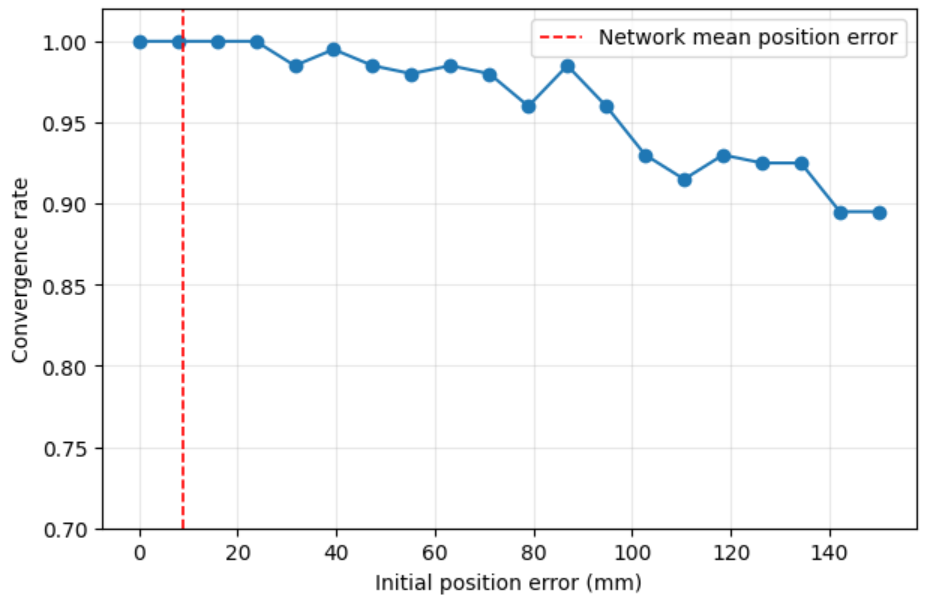
\includegraphics[width = 0.8 \textwidth]{figs/pos_sweep.png}
  \caption{Convergence rate against positional perturbation. The dashed line marks the mean positional error of the trained Neural Network.}
  \label{fig:pos_sweep}
\end{figure}

\paragraph{Angular Sweep.} The angle is swept from $\alpha = 0$ to $\alpha = 90^{\circ}$. Figure \ref{fig:angle_sweep} shows the same story as the positional sweep, steady decrease with no sharp dropoff. We do note that the angle is a lot more forgiving than position, retaining a 97.5\% convergence rate up to $\alpha = 42.6^\circ$. This is because the equation \eqref{eq:forward} depends on $1/r^{3}$ whereas the orientation angle only enters through the dot product.

\begin{figure}
  \centering
  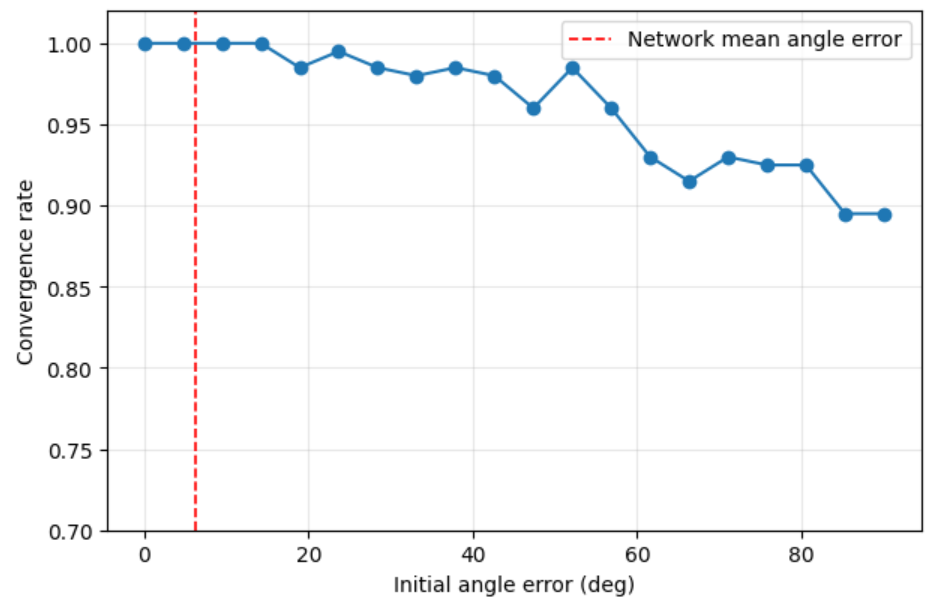
\includegraphics[width = 0.8\textwidth]{figs/angle_sweep.png}
  \caption{Convergence rate against angular perturbation. The dashed line marks the mean angular error of the trained Neural Network.}
  \label{fig:angle_sweep}
\end{figure}

\section{Network Training}
\subsection{Training Configuration}
In training the network, a number of tuning choices were made against the validation set. First, and most importantly, the network uses the 6-dimensional $(x,y,z,n_1,n_2,n_3)$ pose representation rather than the 5-dimensional $(x,y,z,\theta,\phi)$ representation. Secondly the "PoseLoss" loss function described in Section \ref{sec:methods-loss} was used, instead of MSE. Third, the learning rate was varied using a cosine annealing scheduler, as described in section \ref{sec:representation}. Each of these training configurations are shown in  Table \ref{tab:training_config} 
\begin{table}
  \centering
  \begin{tabular}{llllll}
    \toprule
    Name & Target & Loss & LR Scheduler & Optimiser & Epochs\\
    \midrule
    Base & $(\theta,\phi)$ & MSE & None & Adam & 200  \\
    Normal & $\hat{n}$ & MSE & None & Adam & 200\\
    PoseLoss & $\hat{n}$ & PoseLoss & None & Adam & 200 \\
    Final & $\hat{n}$ & PoseLoss & Cosine & Adam & 200 \\
    \bottomrule
  \end{tabular}
  \caption{Experimental Design of NN models.}
  \label{tab:training_config}
\end{table}
\begin{table}
  \centering
  \begin{tabular}{lll}
    \toprule
    Name & Mean Pos Error (mm) & Mean Angular Error (deg)  \\
    \midrule
    Random Pair & 165 & 90 \\
    Centre Predictor & 120 & 90 \\
    Base & 135 & 87.1  \\
    Normal & 139 & 47.7 \\
    PoseLoss & 21.3 & 8.67 \\
    Final & 9.2 & 6.43 \\
    \bottomrule
  \end{tabular}
  \caption{Test set performance of NN models.}
  \label{tab:nn_results}
\end{table}

\paragraph{Base.}Table \ref{tab:nn_results} shows that the base model performs only marginally better than a baseline estimator i.e. it is not much better than a random guess. The expected positional and angular error for two randomly sampled points were estimated using a Monte Carlo simulation drawing from the test set. More interestingly, the base model actually performs worse on position than just guessing the centre of the box every time. This tells us that the base model learns nothing about the orientation and almost nothing about the position.


\paragraph{Normal.}The "Normal" configuration improves the anglular error to about half of baseline but left the positional error the same, suggesting that the change to normal parametrisation allows the network to start learning the orientation configuration of the system.

\paragraph{PoseLoss.}The biggest change happens when we change the loss function from MSE to our PoseLoss, reducing positional error by a factor of 6.5 and angular error b y a factor of 5.5. This change allows the network to actually learn against angular error and also weights the positional and angular error more equally.

\paragraph{Final.}Further refinement is achieved through the use of Cosine learning rate scheduling, allowing training to slow down towards the end, learning the finer details of the data. 
\subsection{Final Model}
The Final NN model, with configuration seen in Table \ref{tab:training_config} was chosen to be used. The number of epochs was chosen to be 200 because by 200 the error on the validation set started plateauing. This plateau can be seen in Figure \ref{fig:training_curves}. 

\begin{figure}
  \centering 
  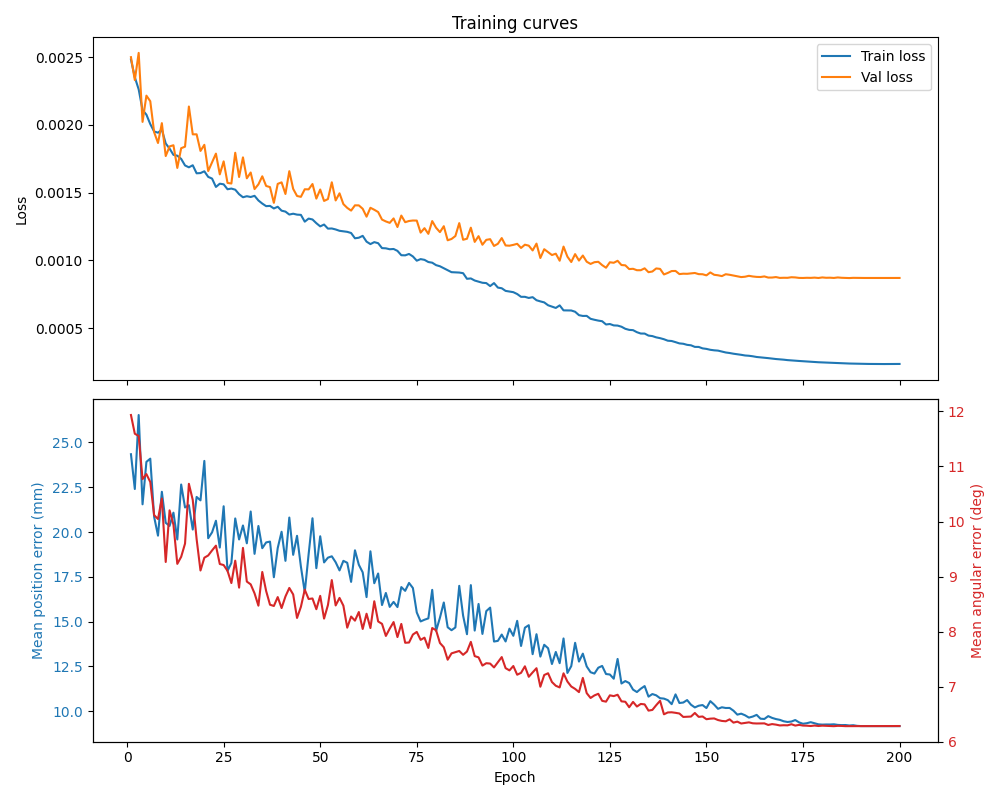
\includegraphics[width = 0.8\textwidth]{figs/training_curves.png}
  \caption{Loss curves and error curves on the validation set}
  \label{fig:training_curves}
 \end{figure}


\subsection{Pose representation}



\section{Three-way Comparison}




